\documentclass[runningheads]{llncs}
\usepackage[english]{babel}
\usepackage[T1]{fontenc}
\usepackage{graphicx}
\usepackage[colorlinks=true, allcolors=blue]{hyperref}
\usepackage{multirow}
\usepackage{float}

\begin{document}

\title{A* and weighted A* algorithms used to solved 8-Puzzle problem - Overview and application}
%
\titlerunning{A* and weighted A* applied to 8-Puzzle}
\author{Alejandro Álvarez Varela UO271288\and
Miguel Menéndez Rodríguez UO269871}
\authorrunning{A. Álvarez, M. Menéndez}
\institute{University of Oviedo, Oviedo, Asturias, Spain
\url{https://www.uniovi.es}}
\maketitle   
\begin{abstract}
In this paper, the aima-java project will be used to test two different algorithms, the A* algorithm, and the Weighted A* algorithm. After a short explanation of said algorithms and the 8-Puzzle problem, which we will be using as an example for this paper, we will experiment on him with different end states and weights, proving that the results go according to the explained theory. To accomplish that, we will be comparing the information acquired after using the different heuristics and algorithms after reaching a solution.
\keywords{A* \and Weighted A* \and 8-Puzzle \and search space \and heuristic}
\end{abstract}

\section{Introduction}
The objective of this paper is to briefly describe the 8-Puzzle problem and to perform an experimental study of some heuristics used to solve this problem with the A* and weighted A* algorithms. It will also explain in more detail how the A* and weighted A* algorithms are applied to the 8-Puzzle problem.
The A* algorithm aims to solve the problem in a way that it always reaches an optimal solution. For that, we'll be using the search spaces and heuristics.
On the other hand, the weighted A* algorithm doesn't go for the best solution, focusing on the states that are closer to the goal.
To appreciate the differences between the two algorithms, we'll be paying attention to the number of expanded nodes, the time used and the cost, the obtained solutions, among many other things, after applying the algorithms to the 8-puzzle problem.
In the end, we'll be comparing all this information, deciding which algorithm, and which heuristic are best for the problem.


\section{8-Puzzle problem}
The 8-Puzzle problem is a widely known problem in the field of Artificial Intelligence. That is due to the fact that, despite its apparent simplicity, it can be very costly for a computer to solve it.
\subsection{Description of the problem}
The 8-Puzzle problem consists on a 3x3 board with 8 tiles labeled from 1 to 8. The goal is to slide the tiles orthogonally to the empty space to match the final configuration. This means that two tiles can not be in the same space, a tile can not pass over another nor can it move diagonally.
Using different algorithms, we'll be searching for the sequence of movements that we'll need to go through to reach the solution, trying to use the less time of execution and number of movements possible.

\section{A* and weighted A* algorithms} \label{s:awa}
a
\subsection{A* algorithm}
a
\subsection{Weighted A* algorithm}
a
\section{A* and weighted A* applied to the 8-Puzzle problem} \label{s:awa8p}
a
\subsection{Heuristics}\label{ss:heuristics}
The heuristics we will be using are the following:
\begin{enumerate}
\item h0: Null heuristic. It is not informed.
\item h1: Weighted misplaced tiles. The number of tiles that are not on the goal location.
\item h2: Weighted Manhattan distance. The Manhattan distance between the goal and the current locations is the sum of the absolute differences of their Cartesian coordinates.
\end{enumerate}
"Weighted" heuristics mean the version of these heuristics for the problem in which the cost of the rules is \(2^i\)

\section{Experimental study}
The following sections will describe the design and results of the study of the two aforementioned algorithms put into practice. This experimental study will be carried out with the heuristics detailed in \ref{ss:heuristics}.
\subsection{Design of the study}
We will try to solve the 8-puzzle problem using the algorithms and heuristics described in \ref{s:awa} and \ref{s:awa8p}. We will measure the time each algorithm takes to run with each heuristic and compare them. Moreover, we will also analyze the number of expanded and reinserted nodes. These samples will be taken from different initial states.
\\
The data were taken in an apparatus with the following characteristics:

\begin{itemize}
\item[$\ast$] Processor: Intel Core i5-6300HQ CPU @ 2.30GHz (4 CPUs)
\item[$\ast$] RAM: 8192MB
\end{itemize}
As mentioned before, the aima-java project will be used with some modifications, such as new heuristics, to collect the data.
\subsection{Experimental results}
Since the heuristic h0 is not informed it will be exactly the same for both the A* and the weighted A* algorithm
\subsubsection{A* algorithm}~\\
The following tables show the number of nodes expanded and reinserted using A* algorithm by each heuristic for the initial states of cost 5, 15 and 30 respectively.

\begin{table}[H]
    \centering
\caption{\label{tab:table1}Number of nodes for the instance \{ 1, 0, 3, 8, 2, 5, 7, 4, 6 \} of cost 5.}
    \begin{tabular}{|c|c|c|c|}
    \hline
       & \multicolumn{3}{|c|}{Heuristic} \\ \hline
        Nodes & h0 & h1 & h2 \\ \hline
        Expanded & 32 & 7 & 5 \\ \hline
        Reinserted & 0 & 0 & 0 \\ \hline
    \end{tabular}
\end{table}

\begin{table}[H]
    \centering
\caption{\label{tab:table2}Number of nodes for the instance \{ 4, 8, 2, 6, 3, 5, 1, 0, 7 \} of cost 15.}
    \begin{tabular}{|c|c|c|c|}
    \hline
       & \multicolumn{3}{|c|}{Heuristic} \\ \hline
        Nodes & h0 & h1 & h2 \\ \hline
        Expanded & 57663 & 1808 & 25 \\ \hline
        Reinserted & 0 & 0 & 0 \\ \hline
    \end{tabular}
\end{table}

\begin{table}[H]
    \centering
\caption{\label{tab:table3}Number of nodes for the instance \{ 5, 6, 7, 2, 8, 4, 0, 3, 1 \} of cost 30.}
    \begin{tabular}{|c|c|c|c|}
    \hline
       & \multicolumn{3}{|c|}{Heuristic} \\ \hline
        Nodes & h0 & h1 & h2 \\ \hline
        Expanded & 175390 & 103737 & 9126 \\ \hline
        Reinserted & 0 & 0 & 0 \\ \hline
    \end{tabular}
\end{table}

\subsubsection{Weighted A* algorithm}~\\
The following tables show the number of nodes expanded and reinserted using weighted A* algorithm by each heuristic for the initial states of cost 5, 15 and 30 respectively.

\begin{table}[H]
    \centering
\caption{\label{tab:table1}Number of nodes for the instance \{ 1, 0, 3, 8, 2, 5, 7, 4, 6 \} of cost 5.}
    \begin{tabular}{|c|c|c|c|}
    \hline
       & \multicolumn{3}{|c|}{Heuristic} \\ \hline
        Nodes & h0 & h1 & h2 \\ \hline
        Expanded & 32 & 7 & 5 \\ \hline
        Reinserted & 0 & 0 & 0 \\ \hline
    \end{tabular}
\end{table}

\begin{table}[H]
    \centering
\caption{\label{tab:table2}Number of nodes for the instance \{ 4, 8, 2, 6, 3, 5, 1, 0, 7 \} of cost 15.}
    \begin{tabular}{|c|c|c|c|}
    \hline
       & \multicolumn{3}{|c|}{Heuristic} \\ \hline
        Nodes & h0 & h1 & h2 \\ \hline
        Expanded & 57663 & 7087 & 47 \\ \hline
        Reinserted & 0 & 429 & 0 \\ \hline
    \end{tabular}
\end{table}

\begin{table}[H]
    \centering
\caption{\label{tab:table2}Number of nodes for the instance \{ 5, 6, 7, 2, 8, 4, 0, 3, 1 \} of cost 30.}
    \begin{tabular}{|c|c|c|c|}
    \hline
       & \multicolumn{3}{|c|}{Heuristic} \\ \hline
        Nodes & h0 & h1 & h2 \\ \hline
        Expanded & 175390 & 102031 & 5623 \\ \hline
        Reinserted & 0 & 21845 & 1369 \\ \hline
    \end{tabular}
\end{table}

\begin{figure}[H]
    \centering
    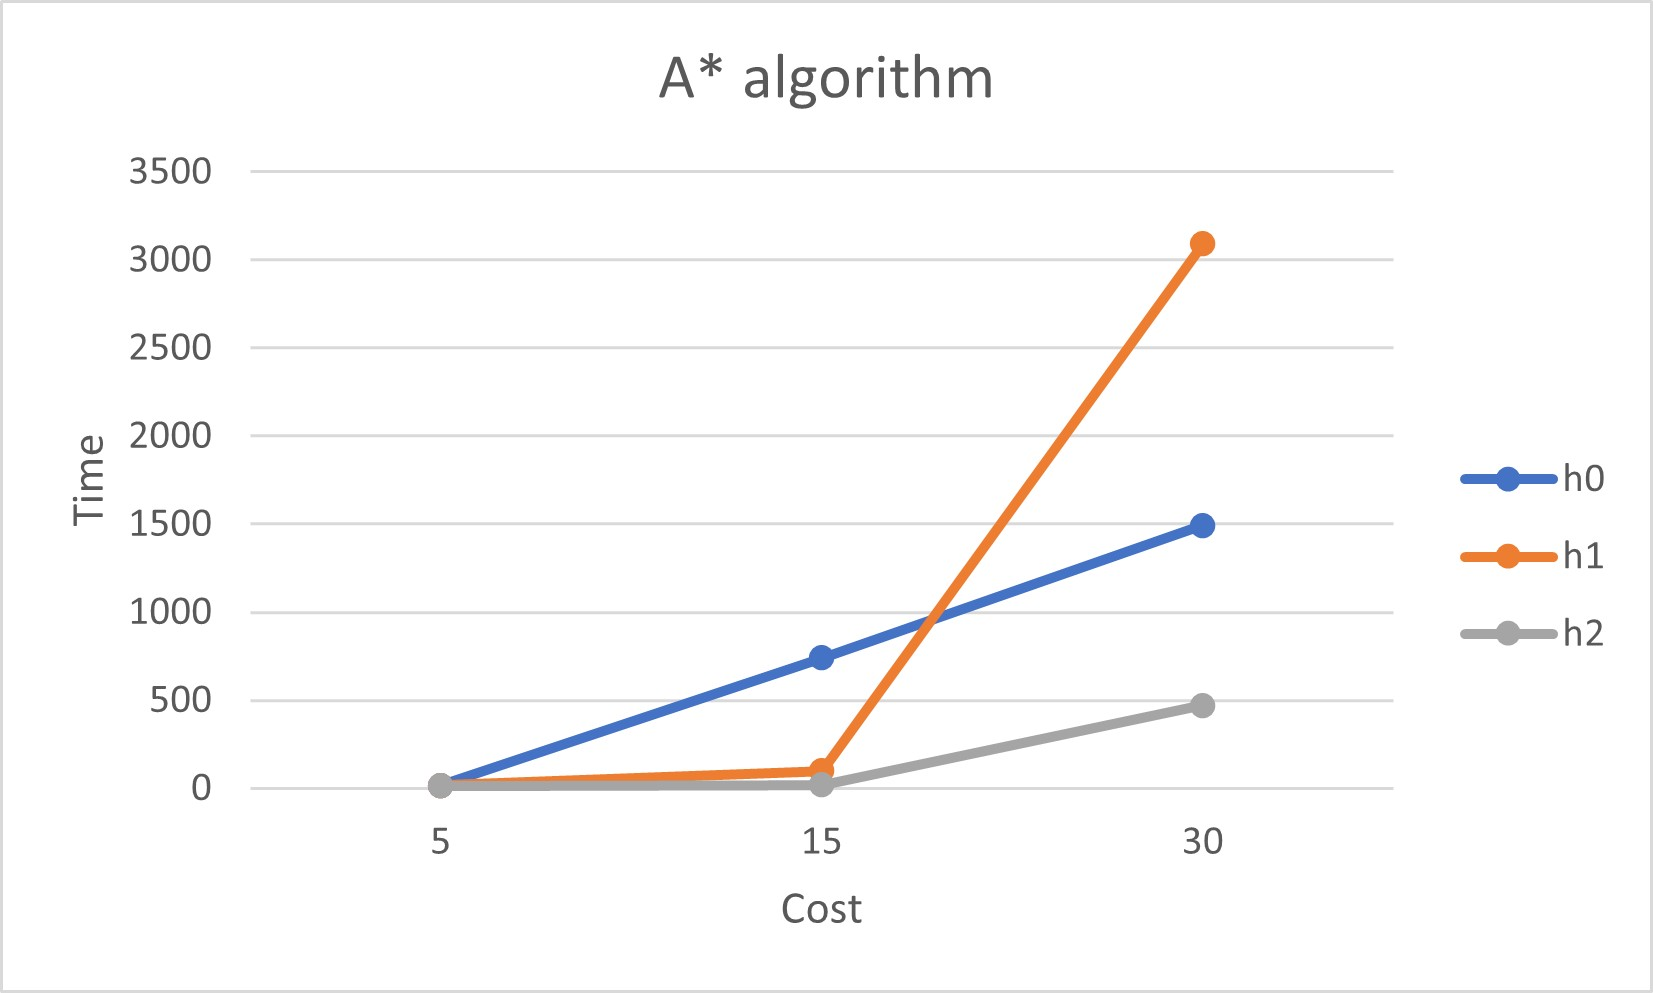
\includegraphics{AStarTimes.jpg}
    \caption{a nice plot}
    \label{fig:mesh1}
\end{figure}

\begin{figure}[H]
    \centering
    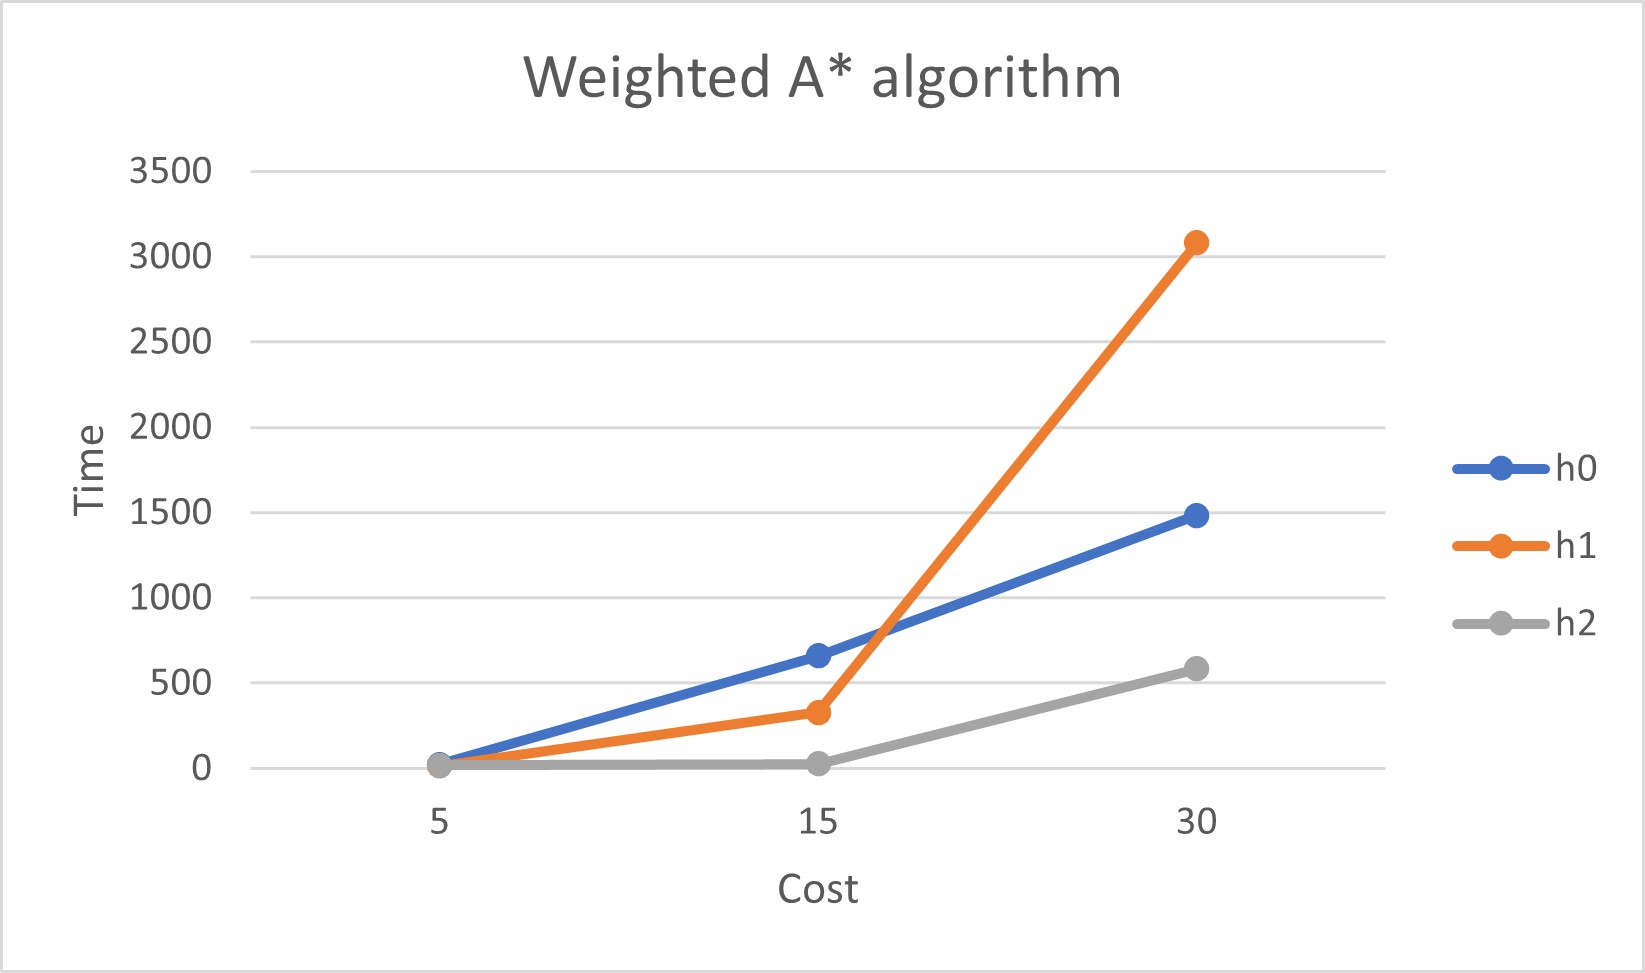
\includegraphics{WeightedAStarTimes.jpg}
    \caption{a nice plot}
    \label{fig:mesh1}
\end{figure}

\section{Conclusion}
a
\section*{Acknowledgments}
We would like to thank the professors of the Intelligent Systems course for giving us the tools and knowledge necessary to carry out this study.
\section*{Appendix A. Contributions}
Alejandro Álvarez was in charge of the measurements of the algorithms, the comparisons between the heuristics and their definitions. He also wrote the section dedicated to the experimental study.
\\
Miguel Menéndez was in charge of writing the introduction to this paper, describing the 8-puzzle problem and the algorithms used during the study.
\\
Finally, the conclusions reached after the completion of this work were drawn by both members.

%
%
%\noindent Displayed equations are centered and set on a separate
%line.
%\begin{equation}
%x + y = z
%\end{equation}
%Please try to avoid rasterized images for line-art diagrams and
%schemas. Whenever possible, use vector graphics instead (see
%Fig.~\ref{fig1}).
%
%%\begin{figure}
%%\includegraphics[width=\textwidth]{fig1.eps}
%%\caption{A figure caption is always placed below the illustration.
%%Please note that short captions are centered, while long ones are
%%justified by the macro package automatically.} \label{fig1}
%%\end{figure}
%
%\begin{theorem}
%This is a sample theorem. The run-in heading is set in bold, while
%the following text appears in italics. Definitions, lemmas,
%propositions, and corollaries are styled the same way.
%\end{theorem}
%
%\begin{proof}
%Proofs, examples, and remarks have the initial word in italics,
%while the following text appears in normal font.
%\end{proof}
%For citations of references, we prefer the use of square brackets
%and consecutive numbers. Citations using labels or the author/year
%convention are also acceptable. The following bibliography provides
%a sample reference list with entries for journal
%articles~\cite{ref_article1}, an LNCS chapter~\cite{ref_lncs1}, a
%book~\cite{ref_book1}, proceedings without editors~\cite{ref_proc1},
%and a homepage~\cite{ref_url1}. Multiple citations are grouped
%\cite{ref_article1,ref_lncs1,ref_book1},
%\cite{ref_article1,ref_book1,ref_proc1,ref_url1}.
%


%
% ---- Bibliography ----
%
% BibTeX users should specify bibliography style 'splncs04'.
% References will then be sorted and formatted in the correct style.
%
%\bibliographystyle{splncs04}
%\bibliography{mybibliography}
%%
%\begin{thebibliography}{8}
%\bibitem{ref_article1}
%Author, F.: Article title. Journal \textbf{2}(5), 99--110 (2016)
%
%\bibitem{ref_lncs1}
%Author, F., Author, S.: Title of a proceedings paper. In: Editor,
%F., Editor, S. (eds.) CONFERENCE 2016, LNCS, vol. 9999, pp. 1--13.
%Springer, Heidelberg (2016). \doi{10.10007/1234567890}
%
%\bibitem{ref_book1}
%Author, F., Author, S., Author, T.: Book title. 2nd edn. Publisher,
%Location (1999)
%
%\bibitem{ref_proc1}
%Author, A.-B.: Contribution title. In: 9th International Proceedings
%on Proceedings, pp. 1--2. Publisher, Location (2010)
%
%\bibitem{ref_url1}
%LNCS Homepage, \url{http://www.springer.com/lncs}.
%\end{thebibliography}
\end{document}
